\section{Příklad 2}
% Jako parametr zadejte skupinu (A-H)
\druhyZadani{F}

Sečteme vnitřní odpor $R_{12345}$ neboli $R_i$:
$$R_{23} = R_2 + R_3 = 350 + 600 = 950\Omega$$
    \begin{figure}[htb]
    \centering
    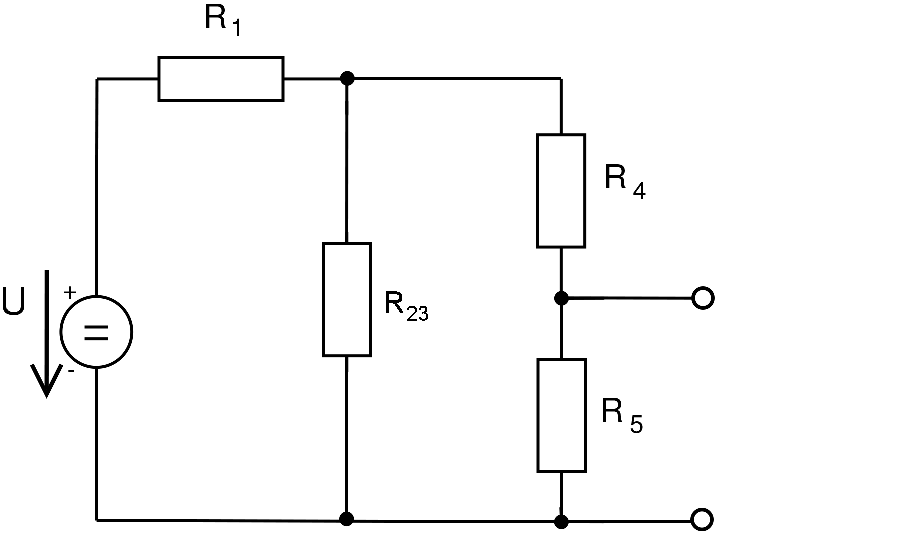
\includegraphics[scale=0.5,keepaspectratio]{sablona/fig/Pr2_Rezistor23.pdf} \\
    \caption{Sečtení $R_2$ a $R_3$}
    \end{figure}
\newpage

$$R_{123} = \frac{R_1*R_{23}}{R_1+R_{23}} = \frac{180*950}{180+950} = 151,3274336\Omega$$
\begin{figure}[htb]
    \centering
    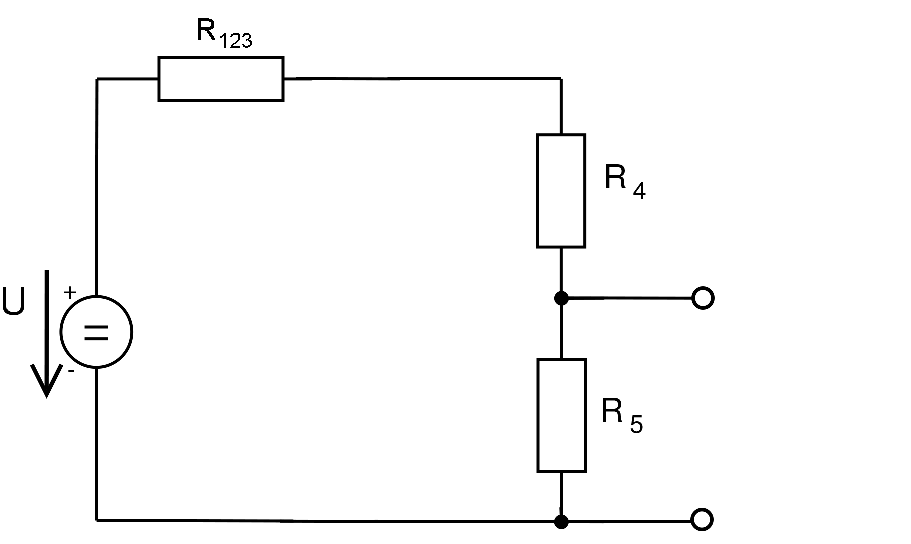
\includegraphics[scale=0.5,keepaspectratio]{sablona/fig/Pr2_Rezistor123.pdf} \\
    \caption{Sečtení $R_1$ a $R_{23}$}
    \end{figure}
    
$$R_{1234} =  R_{123} + R_4 = 151,3274336 + 195 = 346,3274336\Omega$$
\begin{figure}[htb]
    \centering
    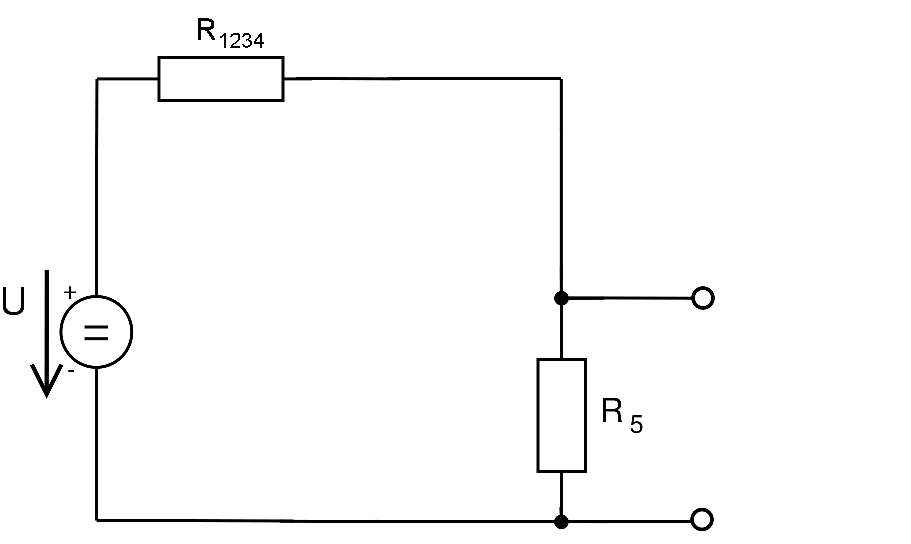
\includegraphics[scale=0.5,keepaspectratio]{sablona/fig/Pr2_Rezistor1234.pdf} \\
    \caption{Sečtení $R_{123}$ a $R_{4}$}
    \end{figure}
    
$$R_{12345} = R_i = \frac{R_{1234}*R_5}{R_{1234}+R_5}= 225,9426211\Omega$$
\begin{figure}[htb]
    \centering
    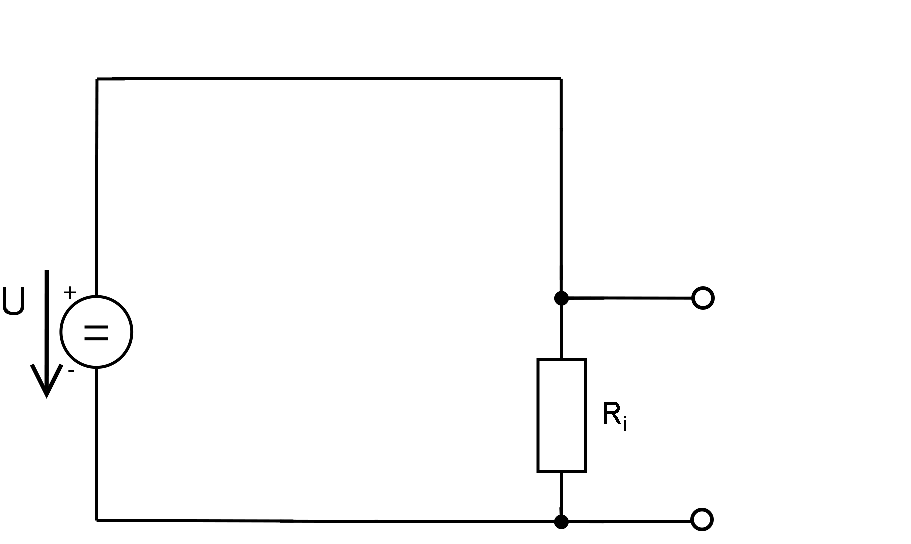
\includegraphics[scale=0.5,keepaspectratio]{sablona/fig/Pr2_Rezistor_i.pdf} \\
    \caption{Sečtení $R_{1234}$ a $R_{5}$}
    \end{figure}
\newpage
Pro výpočet $U_i$ využijeme metodu smyčkových proudů:
\begin{figure}[htb]
    \centering
    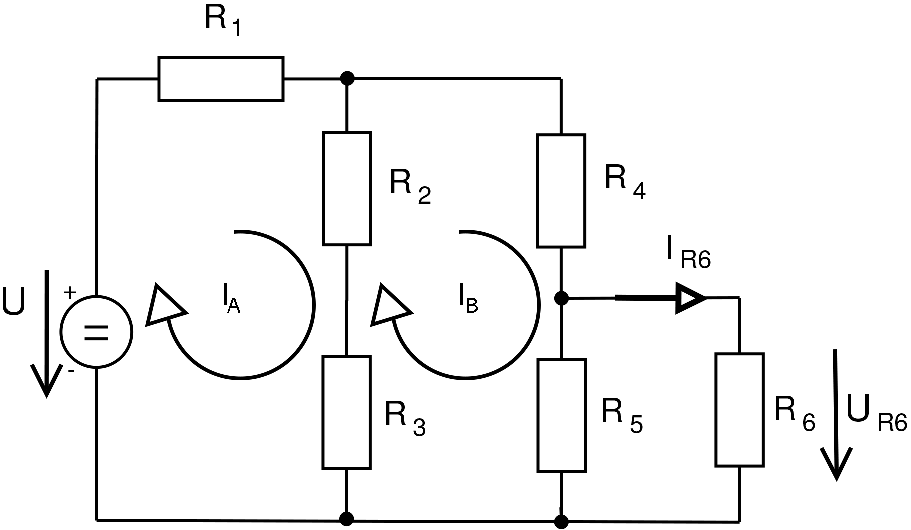
\includegraphics[scale=0.5,keepaspectratio]{sablona/fig/Pr2_Smycky.pdf} \\
    \caption{Vyznačení smyčkových proudů}
    \end{figure}

Vypočítáme si proud $I_B$ dosazením rovnice přímo do matice:
\[
\left(
\begin{array}{cc}
R_1 +R_{23} & -R{23}\\
-R{23} & R_4+R_5+R_{23}\\
\end{array}
\right)
*
\left(
\begin{array}{c}
I_A\\
I_B\\
\end{array}
\right)
=
\left(
\begin{array}{c}
U\\
0\\
\end{array}
\right)
\]
\[
\left(
\begin{array}{cc}
1130 & -950\\
-950 & 1795\\
\end{array}
\right)
*
\left(
\begin{array}{c}
I_A\\
I_B\\
\end{array}
\right)
=
\left(
\begin{array}{c}
130\\
0\\
\end{array}
\right)
\]
\newline

Vypočítáme determinanty za pomoci křížového pravidla pro výpočet determinantů:
\[
D = 
\left|
\begin{array}{cc}
1130 & -950\\
-950 & 1795\\
\end{array}
\right|
= 11258500
\]
\newline
\[
D_2 = 
\left|
\begin{array}{cc}
1130 & 130\\
-950 & 0\\
\end{array}
\right|
= 123500
\]
\newline

Využijeme Cramerovo pravidlo a vypočítáme smyčkový proud $I_B$:
$$I_B = \frac{D_2}{D} = \frac{11258500}{123500} = \frac{2470}{225517}A$$
$$U_i = U_{R_5} = I_B*R_5 = \frac{2470}{22517}*650 = 71,301683172713985V$$
\newpage

\begin{figure}[htb]
    \centering
    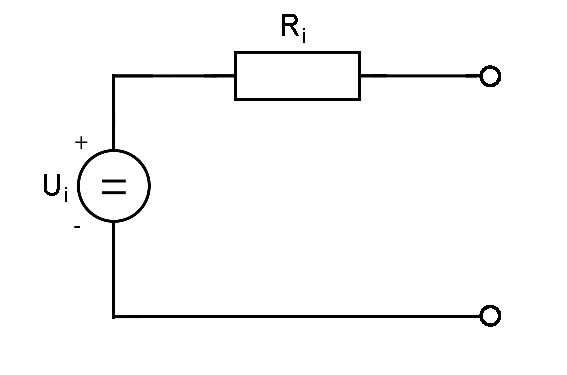
\includegraphics[scale=0.5,keepaspectratio]{sablona/fig/Pr2_Ui_Ri.pdf} \\
    \caption{Náhradní obvod s $U_i$ a $R_i$}
    \end{figure}

$$I_{R_4} = \frac{U_i}{R_i + R_4} = \frac{71,301683172713985}{225,9426211} = \mathbf{0,2330557374A}$$
$$U_{R_6} = R_6*I_{R_6} = 80 *  2290264981 = \mathbf{18,64445899V}$$